\chapter{Strumenti fondamentali} \label{tools}
Prima di addentrarci nella trattazione del teorema, richiamiamo alcune nozioni alla base di quanto diremo più avanti. 
In particolare, avere chiare queste informazioni risulterà cruciale per assicurarsi di aver compreso a fondo il significato delle ipotesi che richiederemo e le tecniche dimostrative utilizzate.

Prima di tutto, anche per cominciare a prendere familiarità con la notazione, ripassiamo la nomenclatura delle equazioni equazioni differenziali di ordine $k$, e di conseguenza degli operatori ad esse associate, con una tabella riassuntiva:
\vspace{5mm}
\begin{center}
\renewcommand{\arraystretch}{2}
\begin{tabular}{l l} 
\hline \hline
 Lineare & $\sum_{|\alpha |\leq k} a_\alpha \, D^\alpha u = f$ \\
 \hline
 \vspace{-2mm}
 Quasi-lineare & $\sum_{|\alpha |= k} a_\alpha (x,D^\beta u) \, D^\alpha u +  a_0(x,D^\beta u)= f,$\\
 & $\quad |\beta |<k $ \\
 \hline
 Non lineare & $F(x,D^\alpha u)=0, \quad |\alpha | \leq k$ \\
 \hline
 In forma normale & $D_{t}^k u = G(x,t, D^\alpha_x D^j_t u), \quad |\alpha |+j \leq k, \, j < k$ \\
 \hline \hline
\end{tabular}
\end{center}
\vspace{5mm}
\begin{remark}
Da qui in poi non faremo sempre particolare attenzione alle assunzioni di regolarità dei dati delle equazioni ($f,a_\alpha,F,G$ e altro), poiché ai nostri scopi è sufficiente che le affermazioni siano vere nel caso in cui tutto sia assunto analitico (con un certo raggio di convergenza). In ogni caso, quando non specificato, la regolarità può essere considerata come almeno $C^1$.
\end{remark}
\begin{remark}
Nel caso di equazione in forma normale si dividono le variabili tra spazio $x\in \mathbb{R}^{n-1}$ e tempo $t$, per una ragione che sarà chiara una volta conclusa la lettura di questo capitolo.
\end{remark}
Cominciamo già ad anticipare che, successivamente, i coefficienti e le funzioni che definiscono le equazioni li assumeremo molto regolari, per la precisione analitici (ovvero localmente sviluppabili in serie di potenze).
\newpage
Alla luce di quanto detto fin'ora, ci rendiamo conto di come ci sarebbero già alcuni aspetti su cui sarebbe importante soffermarsi.
Ma per essere più ordinati riassumiamo le nostre tematiche di interesse in quattro punti, i quali rispecchiano la struttura dei questo capitolo:
\begin{enumerate}
\item \textbf{superfici caratteristiche}: ovvero quelle superfici in $\mathbb{R}^n$ che sono strettamente legate alla forma dell'equazione in osservazione e che possono essere fonte di problemi quando si decide di assegnare dei dati Cauchy su di esse;
\item \textbf{metodo delle caratteristiche}: nel caso di equazioni, anche non lineari, del primo ordine è possibile vedere un'EDP come un sistema di EDO dipendente da un parametro;
\item \textbf{problemi di Cauchy}: l'unica tipologia di problemi di cui ci occuperemo;
\item \textbf{serie di potenze}: costituiscono le fondamenta del concetto di funzione analitica (e olomorfa nel caso dei numeri complessi), ovvero l'unica tipologia di funzioni che cercheremo come soluzione. 
\end{enumerate}


\section{Superfici caratteristiche}
In questa prima sezione introduciamo il concetto di superficie caratteristica nei casi più semplici, in modo da comprenderne a pieno il significato. Cominciamo mettendoci nella situazione più semplice in assoluto, ovvero quella di un'equazione lineare. 
Tale equazione è univocamente determinata dal termine forzante che abbiamo chiamato $f$ e da un operatore differenziale lineare $L=\sum_{|\alpha |\leq k} a_\alpha \, D^\alpha$. Concentriamo la nostra attenzione su quest'ultimo e diamo tre definizioni.

\begin{definition}
Forma caratteristica di $L$:  $\chi_L(x,\xi)=\sum_{|\alpha |= k} a_\alpha(x) \, \xi^\alpha$ con  $x,\xi \in \mathbb{R}^n$.
\end{definition}

\begin{definition}
Varietà caratteristica di $L$ in $x$: $\text{char}_x (L)= \{ \xi \neq 0 : \chi_L(x,\xi)=0 \}$.
\end{definition}

\begin{definition}
$\Gamma$ superficie caratteristica per $L$ in $x \iff \nu(x) \in\text{char}_x (L)$.
\end{definition}

Cerchiamo ora di indagare il significato di queste definizioni:
\begin{itemize}
\item Prima di tutto notiamo che quando $\xi \in \text{char}_x (L)$ è come se l'operatore non fosse ``propriamente'' di ordine $k$ nella direzione $\xi$.
\item Inoltre nel caso di operatore del primo ordine ($k=1$), una superficie $\Gamma$ è caratteristica quando $A=(a_1,\ldots ,a_n)$ è tangente a $\Gamma$ punto per punto (ovvero per ogni $x\in \Gamma$).
\item E' possibile dimostrare che una superficie caratteristica ``porta con sé più informazioni'' nel momento in cui si assegnano delle condizioni di Cauchy su di essa. Infatti, note le derivate normali $D^i_\nu u \,(i<k)$ di una funzione $u$ che vogliamo soddisfi l'equazione, nel caso in cui $\Gamma$ non sia caratteristica in ogni punto, è possibile calcolare tutte le derivate parziali di $u$ su $\Gamma$.
\end{itemize}
\newpage
Specialmente l'ultima considerazione, a causa della scarsa rigorosità, potrebbe essere fonte di confusione ad una prima lettura. Esiste però un teorema, che mostra tale risultato in modo esplicito nel caso di equazioni quasi-lineari e che può essere trovato insieme alla dimostrazione in \cite[cap.4.6]{Evans}.

Considerando che ambiamo a dimostrare un teorema che si rivelerà molto generale, notiamo che, purtroppo, le equazioni lineari non saranno sufficienti a risolvere tutti i nostri problemi. Per questo motivo, vogliamo generalizzare immediatamente il concetto di superficie non caratteristica al caso quasi-lineare, anche se rimaniamo nel caso di equazione del primo ordine. 

Supponendo di avere il problema di Cauchy
\begin{equation}
\begin{cases}
\sum a_j(x,u)D_{x_j} u = b(x,u)\\
u = \phi \text{ su } \Gamma
\end{cases}
\end{equation}
e che $\Gamma$ abbia come parametrizzazione locale in un intorno di $x_0\in \Gamma$ la funzione $\gamma (s): \mathbb{R}^{n-1}\rightarrow \mathbb{R}^n$, forniamo la seguente generalizzazione, chiaramente ispirata al caso di operatori lineari del primo ordine.
\begin{definition}
$\Gamma$ non caratteristica in $x_0=\gamma (s_0)$ se e solo se\\
\begin{equation*}
\det
\underbrace{
\left[
\begin{matrix}
D_{s_1}\gamma_1 & \cdots & D_{s_{n-1}}\gamma_1 \\
\vdots &  & \vdots \\
D_{s_1}\gamma_n & \cdots & D_{s_{n-1}}\gamma_n \\
\end{matrix}\;\right|}_{\text{span del piano tangente}} \,
\left.
\begin{matrix}
a_1(\gamma, \phi(\gamma))\\
\vdots\\
a_n(\gamma, \phi(\gamma))\\
\end{matrix}\right] (s_0) \neq 0
\end{equation*}
\end{definition}
Adesso è arrivato il momento di utilizzare queste definizioni per trarre qualche conseguenza utile.

\newpage
\section{Metodo delle caratteristiche}
I problemi seguenti sono \textbf{equivalenti}.
\begin{equation} \label{edpquasilin}
\text{EDP : }
\begin{cases}
\sum a_j(x,u)D_{x_j} u = b(x,u)\\
u = \phi \text{ su } \Gamma
\end{cases} 
\end{equation}
\begin{equation}
\text{EDO : }
\begin{cases}
D_t \, x = A(x,y) \; \footnotemark \\
D_t \, y = b(x,y)\\ 
x(0)=x_0\\ 
y(0) = \phi (x_0) \quad \forall x_0 \in \Gamma
\end{cases} 
\end{equation}
Dove $y = u(x)$ e $A(x,y)=[a_1(x,y),\ldots ,a_n(x,y)]$.
\footnotetext{le soluzioni $x$ vengono dette \textit{curve caratteristiche}}


\begin{theorem}
\hpth{
\text{Problema \eqref{edpquasilin} } \\
a_j, \, b, \, \phi , \, \Gamma \in C^1\\
\Gamma \text{ non caratteristica}
}{
\exists ! \text{ soluzione } C^1 \text{ in un intorno di } \Gamma
}
\end{theorem}
\begin{proof}
sfruttando il teorema di esistenza e unicità locale per EDO
\end{proof}

si può generalizzare tutto (superfici caratteristiche e metodo delle caratteristiche) al caso non lineare (primo ordine), non lo facciamo perché il metodo delle caratteristiche ci servirà solo nel caso quasi lineare e per la def di non caratteristicità seguiamo un altro approccio più rapido ed equivalente.

\newpage
\section{Problemi di Cauchy}
\begin{itemize}
\item Spesso utilizzato quando la superficie dei dati \textbf{non} è un bordo.
\item Necessita anche le \textbf{derivate normali} ($D^j_\nu u$) della soluzione sulla superficie per determinarla univocamente.
\item Porta con sé il rischio di essere \textbf{sovradeterminato} (buono per l'unicità e meno per l'esistenza della soluzione).
\end{itemize}

Non ci preoccupiamo della regolarità delle funzioni perché poi le assumeremo analitiche.
Problema generale
\begin{equation*}
\begin{cases}
F^*(x,D^\alpha u^*)=0 & |\alpha | \leq k, \, F^* \text{ almeno } C^1\\
D^j_\nu u^* = \phi_j^* & \text{su } \Gamma^* \text{ per }j<k 
\end{cases}
\end{equation*}



Mappatura in $t=0$

Detta $\gamma^*$ la parametrizz. locale di $\Gamma^*$, applichiamo la mappa:
$$\Phi (x) = 
\begin{bmatrix}[ccc|c]
x_1 & \cdots & x_{n-1} & x_n-\gamma^* (x_1,\ldots , x_{n-1})
\end{bmatrix}$$
\begin{figure}[H]
\centering
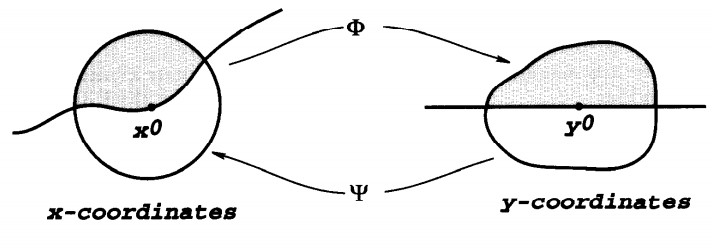
\includegraphics[scale=.5]{flatb}
\caption{Immagine da \cite[cap.8]{Evans}}
\end{figure}



\begin{enumerate}
\item Selezioniamo una variabile privilegiata e chiamiamola ``tempo'':
\begin{align*}
t & \leftarrow x_n \\
x & \leftarrow (x_1,\ldots , x_{n-1})
\end{align*}
\item Chiamiamo $\Gamma_0 = \{t=0\}$.
\item Indichiamo le derivate nel modo seguente: $D^\alpha_x D^j_t u$.
\item Otteniamo il problema ($u^*=u(\Phi)$):
\begin{equation*}
\begin{cases}
F(x,t, D^\alpha_x D^j_t u)=0 & |\alpha | +j \leq k\\
D^j_t u (x,0)= \phi_j(x) & \text{per }j<k 
\end{cases}
\end{equation*}
\end{enumerate}



Superfici non caratteristiche in generale

\begin{definition}
$\Gamma^*$ (o $\Gamma_0$) è non caratteristica $\iff$ l'equazione su $\Gamma_0$ può essere riscritta in \textbf{forma normale} rispetto a $t$.
\end{definition}

\begin{remark}
Si dimostra che è coerente con le definizioni precedenti.
\end{remark}

\begin{remark}
\begin{itemize}
\item Caso lineare $\rightarrow$ condizione sui coefficienti.
\item Caso non lineare $\rightarrow$ validità ipotesi teorema del Dini su $F$.
\end{itemize}
\end{remark}


\newpage
\section{Serie di potenze}
Dando per nota la teoria delle funzioni olomorfe, e di conseguenza anche la teoria base delle funzioni analitiche (reali), in questo paragrafo vogliamo scoprire, o conoscere meglio, solamente degli strumenti molto specifici che ci permetteranno di dimostrare il TCK.

Cominciando dallo studiare uno sviluppo in serie di potenze di una funzione di cui non dobbiamo dimenticarci.
\begin{definition}
Funzione maggiorante: $$\mathcal{M}_{Cr}(x)=\frac{Cr}{r-(x_1+\ldots +x_n)}$$
\end{definition}
Utilizzando il teorema multinomiale, dimostriamo che la questa funzione può essere sviluppata in serie di potenze per $|x|<r/n$, ricavandone l'espressione dei coefficienti $c_\alpha$:
\begin{align*}
\mathcal{M}_{Cr}(x) &= \frac{Cr}{r-(x_1+\ldots +x_n)} = C \sum\limits_{j=0}^\infty \left(\frac{x_1+\ldots +x_n}{r}\right)^j  \\
&= C \sum\limits_{j=0}^\infty \frac{1}{r^j} \sum\limits_\alpha  \binom{|\alpha |}{\alpha } x^\alpha = \sum\limits_\alpha 
\underbrace{C \frac{|\alpha |!}{\alpha ! \, r^{|\alpha |}}}_{c_\alpha} \, x^\alpha .
\end{align*}

A partire da questo risultato, vogliamo enunciare due teoremi, che costituiscono la spina dorsale del cosiddetto metodo dei maggioranti, ideato per la prima volta da Cauchy, e che permettono di giustificare la terminologia introdotta poco fa.

\begin{theorem}[utilità del maggiorante]\label{teomagg}
\hpth{
g_\alpha \geq |f_\alpha|\\
\sum g_\alpha x^\alpha \text{ ha raggio di conv. } R
}{
\sum f_\alpha x^\alpha \text{ha raggio almeno } R
}
\end{theorem}


\begin{theorem}[costruzione del maggiorante]
\hpth{
\sum f_\alpha x^\alpha \text{ ha raggio } R
}{
\exists \, r<R, \, C>0 : \, |f_\alpha | \leq C \frac{|\alpha |!}{\alpha ! \, r^{|\alpha |}}
}
\end{theorem}

\begin{proof}
E' sufficiente notare che prendendo $C \geq |f_\alpha r^{|\alpha |}|$ si ha come conseguenza immediata che
$$|f_\alpha | \leq C \frac{1}{r^{|\alpha |}} \leq C \frac{|\alpha |!}{\alpha ! \, r^{|\alpha |}}.$$
\end{proof}

Nel caso in cui valgano le ipotesi del teorema \ref{teomagg} scriveremo:  $\sum g_\alpha x^\alpha \gg \sum f_\alpha x^\alpha$.

\begin{remark}
Gli stessi teoremi continuano a valere nel caso dei numeri complessi.
\end{remark}
\newpage
\section{Note}
Cosa si intende per superficie analitica\\
superfici caratteristiche e calcolo di tutte le derivate parziali:
\begin{itemize}
\item caso $t=0$
\item caso generale 
\end{itemize}

